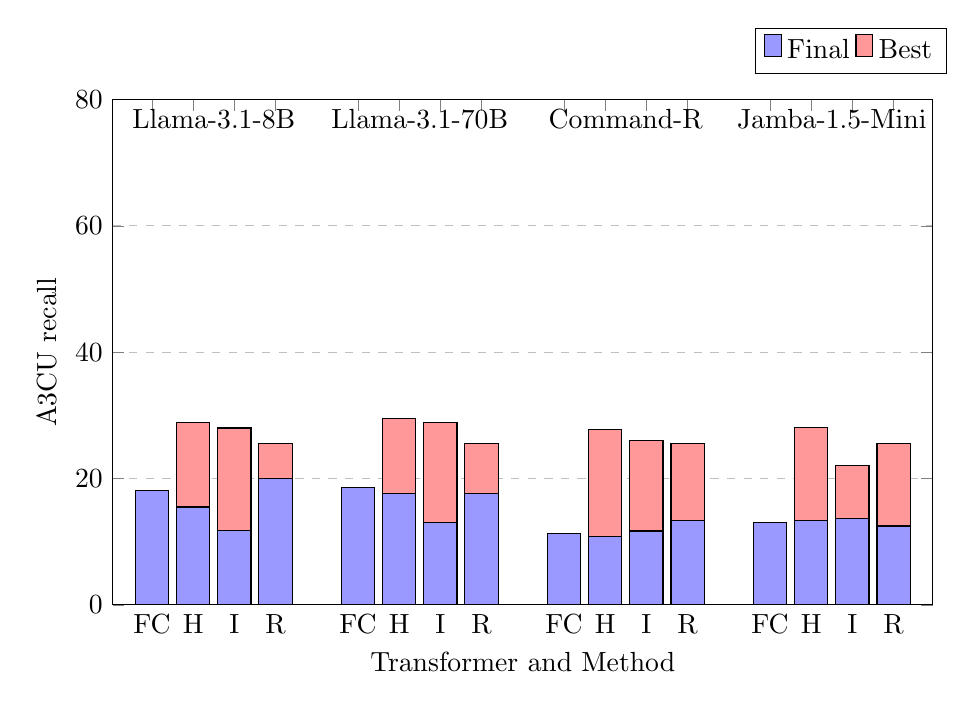
\begin{tikzpicture}
    \begin{axis}[
     width=12cm,
     height=8cm,
     ybar stacked,
     bar width=12pt,
     ylabel={A3CU recall},
     xlabel={Transformer and Method},
     xticklabels={
     FC, H, I, R,
     FC, H, I, R,
     FC, H, I, R,
     FC, H, I, R
     },
     xtick={0,1,2,3,5,6,7,8,10,11,12,13,15,16,17,18},
     x tick label style={anchor=north},
     legend style={at={(0.9,1.05)},anchor=south,legend columns=-1},
     ymajorgrids=true,
     grid style=dashed,
     ymin=0,
     ymax=80,
     enlarge x limits={abs=0.5cm},
    ]
    \addplot[fill=blue!40] coordinates {
     (0,18.1) (1,15.5) (2,11.8) (3,20.0)
     (5,18.6) (6,17.6) (7,13.0) (8,17.6)
     (10,11.3) (11,10.8) (12,11.7) (13,13.3)
     (15,13.1) (16,13.4) (17,13.7) (18,12.5)
     };
    \addplot[fill=red!40] coordinates {
     (0,0) (1,13.4) (2,16.2) (3,5.6)
     (5,0) (6,11.9) (7,15.9) (8,8.0)
     (10,0) (11,17.0) (12,14.3) (13,12.2)
     (15,0) (16,14.7) (17,8.4) (18,13.0)
     };
    \legend{Final, Best}
    \node[anchor=north] at (axis cs:1.5,80) {Llama-3.1-8B};
    \node[anchor=north] at (axis cs:6.5,80) {Llama-3.1-70B};
    \node[anchor=north] at (axis cs:11.5,80) {Command-R};
    \node[anchor=north] at (axis cs:16.5,80) {Jamba-1.5-Mini};
    \end{axis}
\end{tikzpicture}